\documentclass[12pt,a4paper]{report}
\usepackage{minted}
\usepackage[brazil]{babel}
\usepackage[utf8]{inputenc}
\usepackage[T1]{fontenc}
\usepackage{graphicx}
\usepackage[hyperfootnotes=false]{hyperref}
\usepackage{fancyvrb}
\usepackage{float}
\usepackage[bottom]{footmisc}
\usepackage{subfig}

\setlength{\parindent}{15pt}
\setlength{\parskip}{1.5ex}
\newcommand{\HRule}{\rule{\linewidth}{0.5mm}}

\begin{document}

\begin{titlepage}
\begin{center}

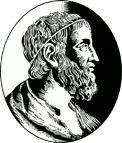
\includegraphics[width=0.15\textwidth]{figuras/grego.jpg}\\[1cm]    
\textsc{\LARGE Instituto de Matemática e Estatística - USP}\\[0.5cm]
\textsc{\large Trabalho final - MAC5742}\\[3cm]
\HRule \\[0.7cm]
{ \huge \bfseries Projeto RAMCloud}\\[0.4cm]

\HRule \\[3.5cm]


\begin{minipage}{0.4\textwidth}
\begin{flushleft} \large
\emph{Autor:}\\
Bruno Padilha\\
\end{flushleft}
\end{minipage}
\begin{minipage}{0.4\textwidth}
\begin{flushright} \large
\emph{Prof.:} \\
Alfredo Goldman vel Lejbman\\
\end{flushright}
\end{minipage}

\vfill

{\large \today}

\end{center}

\end{titlepage}


\begin{abstract}
Desde o início dos anos 80 o disco magnético, também conhecido por disco rígido, hard disk ou HD, é o
principal meio para armazenamento de dados em massa. Embora sua capacidade de armazemento tenha aumentado exponencialmente
ao longo dos anos, acompanhado a evolução dos outro componentes de um PC, seu tempo de acesso e sua taxa de tranferência
de dados pouco evoluiram. Com a crescente demanda por serviços que acessam grandes volumes de dados e a necessidade de se exibir
resultados em tempo real, assim como a queda no preço da memória DRAM, surge a necesidade de se manter cada vez mais dados em memória
volátil. Nesse cenário, o Projeto RAMCloud propõe um sistema de armazenamento de dados inteiramente em memória DRAM, garantido durabilidade,
disponibilidade e baixissima latência de acesso aos dados.
\end{abstract}

\tableofcontents

\chapter{Introdução e Contexto}

A capacidade de armazenar dados em meios eletrônicos cresce exponencialmente desde os primórdios da computação sustentada pelos avanços em pesquisa e tecnologia. 

\par
Os programas de computador, valendo-se desses avanços, também evoluíram e passaram a gerar e manipular um volume cada vez maior de dados que, para serem processados e analisados de modo rápido, eficiente e consistente, passaram a ser armazenados em sistemas especializados denominados Bancos de Dados. 

\par
Os Sistemas de Bancos de Dados viabilizaram a manutenção do histórico dos dados, que além de armazenar os dados e seus respectivos processos de captação, permitem realizar análises estatísticas poderosas como, por exemplo, a detecção de anomalias, agrupamento e predição.

\par
Em geral quanto mais dados se obtém do ciclo de vida de um determinado processo mais precisas serão as análises realizadas sobre os mesmos, porém com um tempo de processamento maior. Esse tempo consumido para a realização das análises de dados muitas vezes é crítico para se tomar uma decisão. O tempo de processamento está diretamente relacionado a estrutura de armazenamento e de relacionamentos dos dados dos sistemas computacionais.

\par 
Um sistema computacional cuja principal finalidade é a analise de dados é denominado sistema analítico, enquanto que um sistema que insere, atualiza, remove, ou seja, modifica constantemente e pontualmente os dados é denominado sistema transacional. Os sistemas analíticos têm como principal característica a consulta a uma grande quantidade de dados com a finalidade de sintetizar ou descobrir informações. 

\par
Se um sistema analítico concorre com um sistema transacional ao acessar os dados, o banco pode sobrecarregar e comprometer a eficiência de ambos os sistemas. Os efeitos colaterais dessa concorrência podem por um lado pode causar a indisponibilidade do sistema transacional e por outro a causar uma lentidão indesejada do sistema analítico. A replicação dos dados em vários níveis é a solução para evitar o problema da concorrência entre o ambiente analítico e o transacional. Essa replicação com alternativas para novas estruturas, tratamento, integração e otimização de acesso aos dados é denominada Data Warehouse.

\par
Para atender a uma importante demanda de análise de dados da Universidade de São Paulo foi criado o projeto denominado DataUSP-PosGrad. Esse projeto propôs a criação de um Data Warehouse com dados de todos os programas da Pós-Graduação e um conjunto de serviços analíticos com o propósito de gerar relatórios sob demanda com análises de tais dados. Esses relatórios incluem análises estatísticas dos programas, áreas e pessoas ligadas à Pós-Graduação, como por exemplo, o número de titulações em uma área, o tempo médio de titulação em um programa, o número de teses dos docentes em uma área ou programa além de muitas outras, publicações e citações.

\par
O principal objetivo deste Trabalho de Conclusão de Curso é o de descrever os principais desafios encontrados e as soluções encontradas para o desenvolvimento de serviços analíticos do Projeto DataUSP-PosGrad.

\section{Problema e Hipótese de solução}

% Hipótese para solucionar o problema de implementação de serviços analíticos (ou seja o uso do REstfull)

O DataUSP-PósGrad precisa ser um sistema escalável, no qual novas funcionalidades podem ser agregadas de maneira simples,
rápida e sem comprometer o seu desempenho. Sua arquitetura deve ser leve e robusta, capaz de manipular um grande volume de dados eficientemente e devolver os resultados ao usuário no menor intervalo de tempo possível, além de ser capaz de fornecer dados a outros sistemas computacionais autonomamente utilizando uma interface web. Para atender a esses requisitos, uma possível solução é construir um conjunto de Web Services sobre a arquitetura RESTful.

\section{Evidências da solução RESTful}

A arquitetura REST separa a implementação de um sistema em cliente e servidor. Essa separação aumenta a escalabilidade do servidor, já que a implementação dos serviços é transparente ao usuário e não mantém estado entre requisições, o que também contribui para um melhor desempenho do sistema como um todo e facilita a incorporação de novos recursos. A interface de acesso aos serviços é homogênea e os recursos disponibilizados são acessados por identificadores únicos (endereços de rede). A arquitetura REST também utiliza o HTTP como protocolo de acesso e não apenas para transporte de dados. Essa interface de acesso utilizará um subconjunto dos métodos do HTTP (GET, POST, PUT, DELETE, etc) para disponibilizar os recursos, simplificando a interação cliente-servidor.

\par
Um Serviço Web, de forma resumida, é uma aplicação que disponibiliza seus recursos por meio de um endereço de rede. Assim qualquer usuário do serviço, seja ele humano ou um programa de computador que conheça o protocolo de comunicação, pode interagir com o mesmo, consumindo seus recursos por meio de troca de mensagens de texto estruturadas. Um Web Service que implementa os conceitos da arquitetura REST sobre o protocolo HTTP é chamado RESTful Web Service.


\section{A arquitetura REST no DataUSP-PósGrad}

A construção do DataUSP-PósGrad sobre a arquitetura REST permite que novas funcionalidades ( em geral a geração de novos relatórios ) sejam implementadas de modo simples e pragmático. O uso do HTTP como protocolo de acesso garante a uniformidade da interface de acesso aos seus recursos, e a aplicação cliente pode ser desenvolvida em diferentes plataformas e sistemas operacionais. Como exemplo de implementação dessa aplicação cliente, pode-se destacar: o uso de  dispositivos móveis ou navegadores de internet garantindo ao sistema uma maior portabilidade a abrangência de uso. Além disso, por haver uma divisão específica entre cliente e servidor parte do processamento pode ser feito do lado cliente, como por exemplo manipular os dados para facilitar a visualização por meio de gráficos ou tabelas, aliviando a carga do servidor e melhorando o desempenho assim como a fluidez geral do sistema.


\section{Descrição dos próximos capítulos}

No capítulo~\ref{ch:2} serão apresentados os fundamentos e conceitos tecnológicos utilizados, tanto na elaboração quanto na construção do sistema DataUSP-PósGrad. O capítulo~\ref{ch:3} descreve as atividades realizadas e as metodologias utilizadas no decorrer do projeto. Já no capítulo~\ref{ch:4} são apresentados os resultados obtidos, com o lançamento oficial do sistema, e os testes de desempenho. No capítulo~\ref{ch:5} constam as conclusões e há uma descrição subjetiva do trabalho no apêncice~\ref{app:a}.   


\chapter{O problema da latência}
\label{ch:2}

\section{Por que a latência importa ?}
A principal motivação do projeto RAMCloud é criar um sistema de armazenamento de dados com uma latência
consideravelmente menor do que os outros sistemas existentes. Tipicamente, aplicações web de larga escala
são executadas em muitos servidores dentro de um \emph{datacenter}, o qual possui máquinas separadas para
executar o código da aplicação e armazenar os dados~\ref{fig:i1}. Quando essa aplicação recebe uma requisição, é necessário
acessar dados que estão no servidor de dados, o que leva de 0.5ms a 10ms. 
\par
Devido à latência de acesso aos dados, uma aplicação que atenda milhões ou até mesmo bilhões de usuários 
não consegue processar muitas requisiçoes de dados aleatórios para uma dada requisição do usuário. Por exemplo, 
para que o Facebook possa ter um tempo de resposta rasoável só é possível que ele faça cerca de 150 requisições
de dados por requisição de usuário (ainda assim utilizando servidores de cache), o que acaba por limitar suas
funcionalidades.   
\par

O propósito do projeto RAMCloud é conseguir prover a menor latência possível para pequenos acessos aleatórios em 
aplicações web de larga escala. Com uma latência de acesso de cerca de 5$\mu$s é uma melhora de 50 a 1000x sobre
os sistemas de armazenamento de dados atuais.


%\begin{figure}[H]
%\begin{minted}[frame=single,linenos,mathescape]{html}
%<!DOCTYPE html>
%<html>
%    <head>
%        <meta charset="UTF-8">
%        <title>Titulo do documento</title>
%    </head>
%    <body>
%        <!-- Conteudo do documento -->
%    </body>
%</html>
%\end{minted}
%\caption{Estrutura básica de um documento HTML}
%\label{lst:html}
%\end{figure}

\begin{figure}[H]\centering
  \centerline{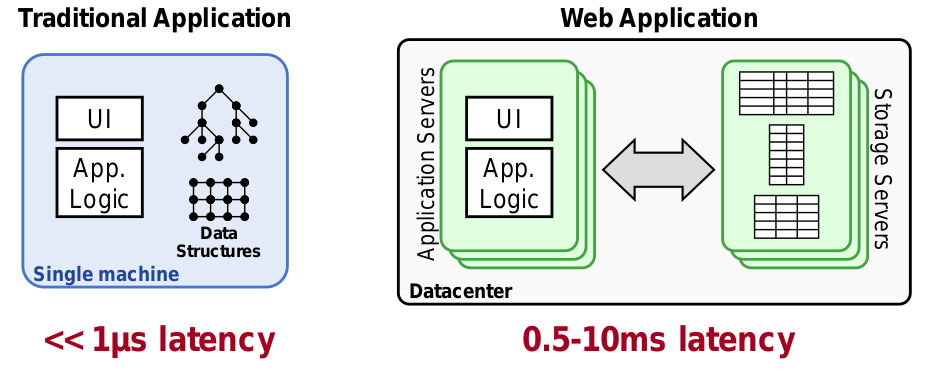
\includegraphics[width=\textwidth]{figuras/i1.png}}
  \caption{Em uma aplicaçao tradicional, os dados e o código estão na mesma máquina (latência de 50-100ns). Já em uma aplicação web escalável, como
  os dados e o código da aplicação estão em máquinas separadas, a latência pode chegar a até 10ms.}\label{fig:i1}
\end{figure}

\section{Atingindo baixa latência}

O principal obstaculo para atingir latências da ordem de 5$\mu$s a 10$\mu$s é a infraestrutura de rede. No início do projeto, no ano de 2009, o tempo típico de uma RPC\footnote{RPC - Remote Procedure Call ou Chamada de procedimento remoto é, basicamente, a operação que permite que um processo possa se comunicar ou outro processo em outra máquina geralmente por meio da rede} era de centenas de $\mu$s~\ref{fig:i2}. Além disso, os prórpios mecanismos do sistema operacional contribuem para aumentar a latência como chamadas ao kernel, a pilha de rede, interrupções, mecanismos de sincronização e o tempo de comunicação entre a CPU e a placa de rede.

\begin{figure}[H]\centering
  \centerline{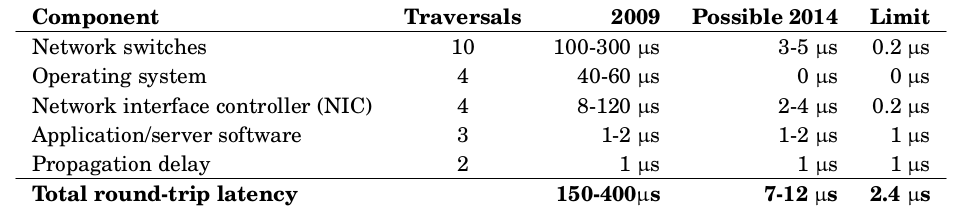
\includegraphics[width=\textwidth]{figuras/i2.png}}
  \caption{Latência média por componente uma uma RPC. \emph{Traversals}: quantas vezes um pacote precisa passar por cada componente em uma 
  requisição completa (round-trip). \emph{2009}: latência típica de um datacenter em 2009. \emph{Possible 2014}: latência possível de se atingir
  em 2014 a um custo razoável.}\label{fig:i2}
\end{figure}

\par

Mesmo com os avanços da tecnologia, a maior parte da latência ainda é gasta na rede ou na placa de rede, o que deixa cerca de 1$\mu$s para o sistema processar cada RPC. Sendo assim, para atingir esse objetivo foi preciso desenvolver um sistema no qual: 
\begin{itemize}
\item Servidores e aplicações precisam enviar e receber pacotes sem passar pelo kernel do sistema operacional;
\item Mecanismos de sincronização precisam ser evitados;
\item Minimizar os erros de coerência de cache;
\item Elimizar os mecanismos de \emph{batching} da placa de rede, onde um certo número de pacotes é acumulado e transmitidos de uma só vez.
\end{itemize}

No RAMCloud os registradores da placa de rede são mapeados diretamente no espaço de memória da aplicação, permitindo uma comunicação direta entre aplicaçao e placa de rede. Além disso, se uma \emph{thread} está esperando pela resposta de uma RPC, ao invés de ir dormir, ela fica constanstemente verificando a placa de rede. Essa técnica, chamada de \emph{busy waiting} (espera ocupada em português), ajuda a minimizar a latência da troca de contexto do sistema operacional.
\par 
Embora a melhor maneira de se minimizar a latência seja utilizar uma única thread para tratar todas as requisições, para garantir a tolerância a falhas os servidores RAMCloud utilizam múltiplas threads: uma única \emph{dispatch thread} e várias \emph{worker threads}. A \emph{dispatch thread} trata de toda a comunicação de rede (requisições e respostas) e também tem a função de selecionar uma \emph{worker thread} para processar cada requisição. Essa comunicação entre threads também é realizada pela técnica de busy waiting. 

\chapter{Arquitetura RAMCloud}
\label{ch:3}


\begin{figure}[H]
\begin{minted}[frame=single,linenos,mathescape,fontsize=\scriptsize,label=exemplo.list]{py3}
# Lista de professores (linhas de comentarios comecam com '#')
4575931307749163,Carlos Hitoshi Morimoto, 1999-HOJE, Professor
0131770792108992,Joao Eduardo Ferreira, 1999-2006 & 2006-HOJE, Professor
0362417828475021,Junior Barrera, 1992-2008, Professor
0926213060635986,Marcel Parolin Jackowski, 2006-HOJE, Professor
0644408634493034,Nina Sumiko Tomita Hirata,,Professor # membro sem periodo
1647118503085126,Roberto Hirata Junior,, Professor # membro sem periodo
2240951178648368,Roberto Marcondes Cesar Junior, 1998-HOJE, Professor
9283304583756076,Ronaldo Fumio Hashimoto,, Professor # membro sem periodo

# lista de colaboradores
4727357182510680,Jesus P. Mena-Chalco, 1995-1999 & 2005-HOJE, Colaborador

# lista de alunos
2837012019824386,Andrea Britto Mattos,, Aluno# membro sem periodo
\end{minted}
\caption{Arquivo de configuração do ScriptLattes que contém a lista de pesquisadores}
\label{lst:slattes}
\end{figure}


\begin{figure}[H]
    \centering 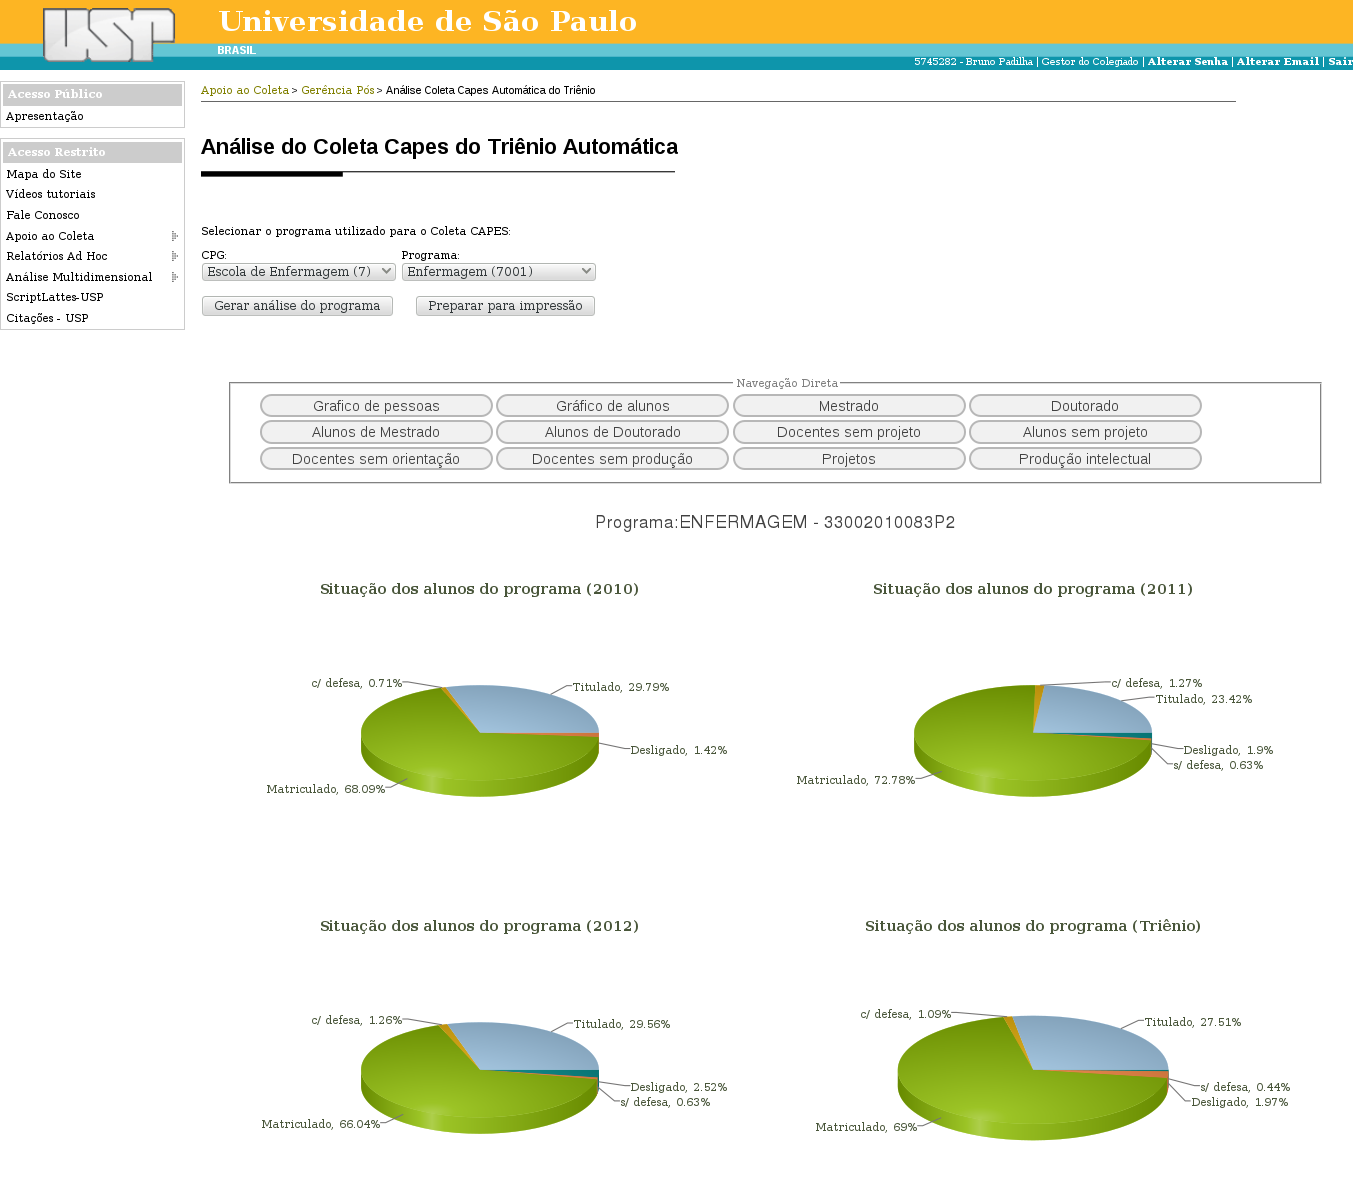
\includegraphics[width=0.5\textwidth]{figuras/trienio.png}
    \caption{Imagem parcial do relatório de análise do triênio}
    \label{fig:trim}
\end{figure} 


\chapter{Resultados e produtos obtidos}
\label{ch:4}

\section{Software final}
O conjunto de ferramentas analíticas desenvolvidas nesse trabalho para auxiliar a tomada de decisões da pró-reitoria
de pós-graduação da USP, recebeu o nome de DataUSP-PósGrad.
\par Sua primeira versão foi lançada oficialmente no dia 05 de junho de 2013, bem recebida pela
comunidade de gestores dos programas de pós-graduação da USP. Ganhou uma matéria na revista \emph{Espaço Aberto} da USP, nas edições 152 e 153\footnote{DataUSP-PósGrad na revista Espaço Aberto - \url{http://espaber.uspnet.usp.br/espaber/?materia=usp-desenvolve-sistema-analitico-de-dados}}.
\par Para capacitar os usuários e apresentar as ferramentas em detalhes, foram realizadas duas oficinas em todos os campus da USP, uma logo após o lançamento~\footnote{1ª oficina DataUSP-PósGrad - \url{http://iptv.usp.br/portal/home.jsp?tipo=0\&\_InstanceIdentifier=0\&\_EntityIdentifier=uspJ3kF6s9CQwQPddjpvikTCs\_sbQicdp
54HCw6bnX8bJs.\&idRepositorio=0\&modelo=0 }} e a segunda na última semana de novembro de 2013.
\par O sistema pode ser acessado por meio do portal \emph{uspdigital} no endereço \emph{http://uspdigital.usp.br/datausppg}. Por disponibilizar informações sensíveis dos programas e dos docentes da USP, o sistema pode ser acessado apenas por um grupo restrito de usuários (Dirigentes de unidades e seus secretários, Reitor, Pró-reitores e alguns outros). Além disso as bases de dados são acessíveis somente de alguns endereços ip específicos, administrados pelo Departamento de Informática da USP.
\par Pelos motivos descritos acima, e também por direitos de produção intelectual, o código do DataUSP-PósGrad pertencente à Pró-Reitoria de Pós-Graduação. O software produzido está em fase de registro pela Diretoria de Informática da Universidade de São Paulo e, uma vez registrado, deverá ser disponibilizado publicamente em forma de serviços.

\section{Teste de Carga}

Algumas consultas aos bancos de dados para gerar os relatórios no DataUSP-PósGrad são expressivamente caras computacionalmente, ou seja, um grande volume de dados precisa ser processado para se obter o resultado. Isso se traduz em tempo de processamento e, por consequência, o usuário do sistema precisa esperar alguns segundos para poder visualizar os dados. Com isso foram elaborados alguns teste de carga, com a finalidade de aferir o tempo de resposta do sistema simulando uma certa quantidade de usuários simultâneos e, poder avaliar a usabilidade como também a sensação de fluidez de DataUSP-PósGrad em uma situação de alta demanda.

\subsection{Metodologia de teste}

Os testes foram realizados com o relatório de Titulações por Ano~\ref{subsub:titano}(Ilustrado no exemplo~\ref{sub:exemplo}). Para cada usuário simulado é sorteada aleatoriamente uma área da pós-graduação para a qual deseja-se exibir o relatório do numero de títulos por ano, no intervalo de 1970 a 2013, do mesmo modo que seria feito utilizando-se a Interface Web. Os resultados são uma média de três repetições de cada teste.
\par
Foram utilizados dois bancos de dados distintos: Sybase ASE versão 13, que é utilizado em produção pelo DataUSP-PósGrad e também pelos demais sistemas administrativos da USP; Microsoft SQL Server versão 11, utilizado para armazenar o modelo multi-dimensional~\ref{sub:multi} e gerar os cubos off-line. 
\par
Para simular a carga de usuários foi utilizado o software JMeter~\footnote{Apache JMeter - http://jmeter.apache.org/}. Além disso, tanto o Servidor de Recursos quanto a Interface Web do DataUSP-PósGrad foram executados na mesma máquina em todos os testes.
\par
O JMeter (figura~\ref{fig:jmeter}) é um software livre da fundação Apache escrito em Java especialmente para realizar testes de carga, aom suporte a diversos tipos de protocolos de rede e dentre eles o HTTP. No caso do DataUSP-PósGrad, o JMeter funciona executando um script que simula as ações de um usuário interagindo com a Interface Web. Esse script pode então ser executado em paralelo simulando um determinado número de usuários. O resultado é um gráfico que exibe a vazão de dados, média, mediana e desvio padrão do tempo de resposta das requisições ao Servidor de Recursos. 
\par
O objetivo desse teste é determinar o impacto da quantidade de usuários simultâneos no desempenho geral do sistema. Atualmente o DataUSP-PósGrad possui cerca de 2000 usuários cadastrados.

\begin{figure}[H]
    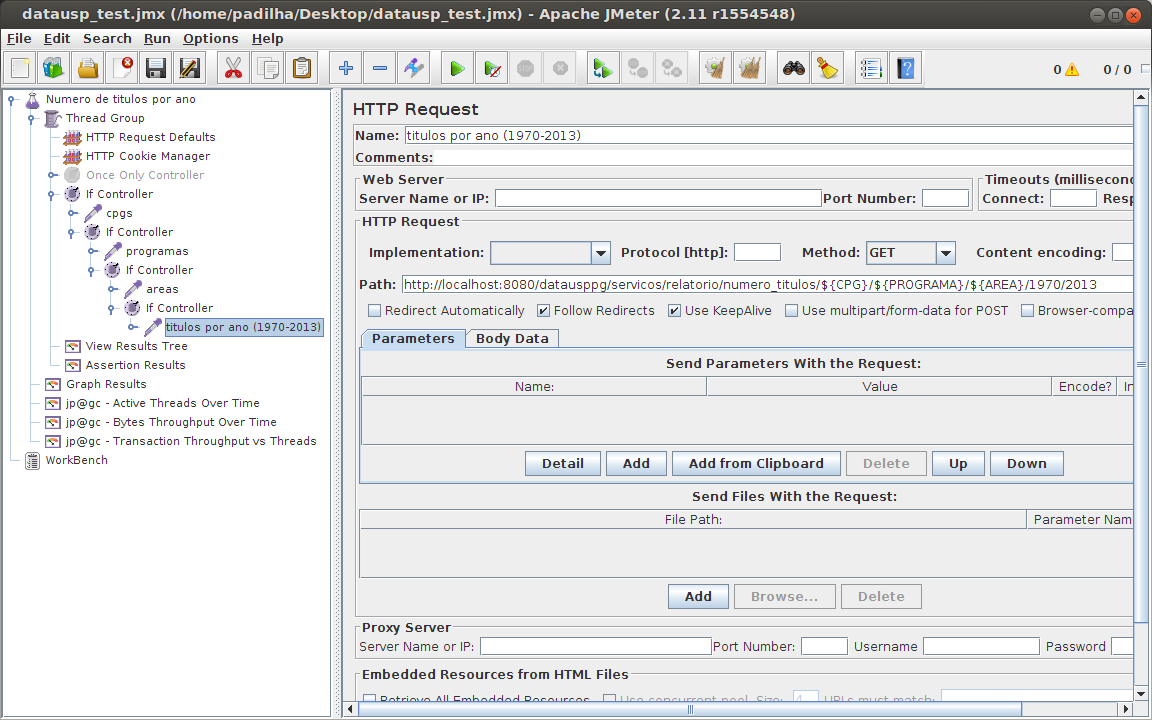
\includegraphics[width=\textwidth]{figuras/jmeter}
    \caption{Interface gráfica do JMeter}
    \label{fig:jmeter}
\end{figure}

\subsection{Resultado dos testes}

Utilizando o banco de dados Sybase ASE foram feitos testes simulando 30, 90 e 360 usuários simultâneos. Os resultados são apresentados nas figuras a seguir.

\begin{figure}[H]
\centering
\subfloat[Sybase ASE]{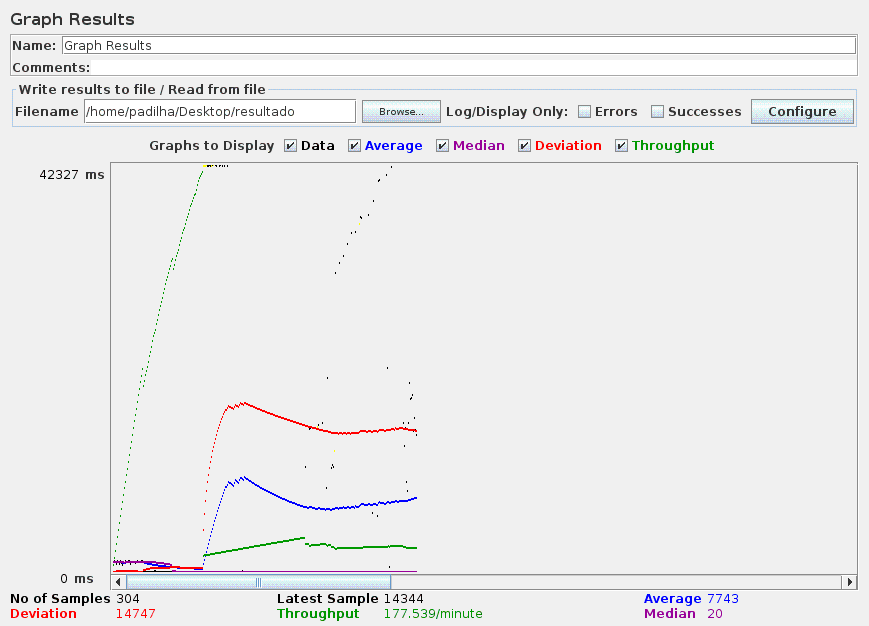
\includegraphics[width=\textwidth]{figuras/psy_30}}\\
\subfloat[MS SQL Server]{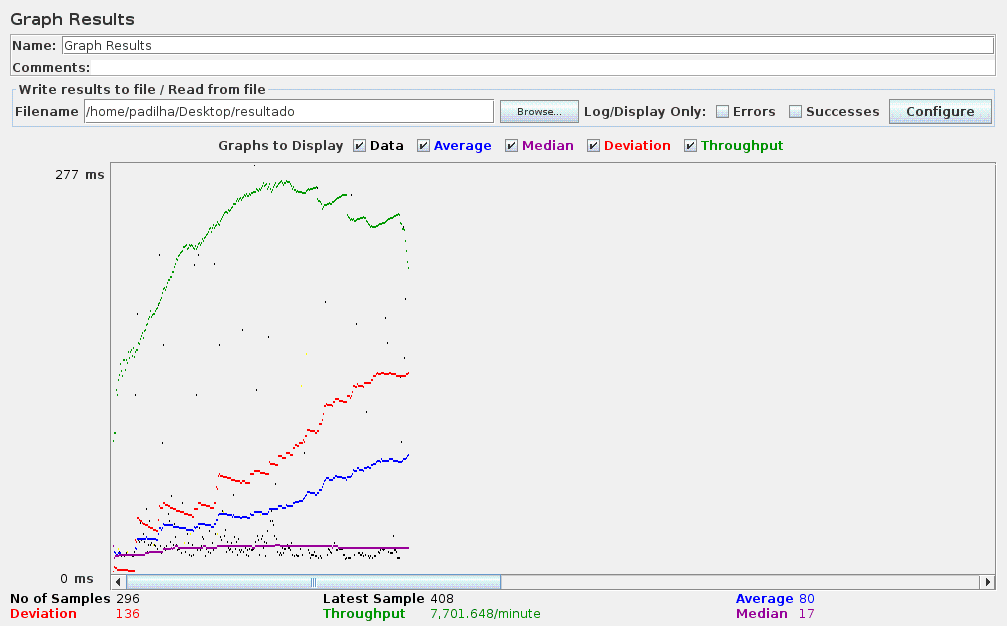
\includegraphics[width=\textwidth]{figuras/pms_30}}
\caption{Gráfico gerado pelo JMeter: 30 usuários}
\label{fig:comp_30}
\end{figure}

\begin{figure}[H]
\centering
\subfloat[Sybase ASE]{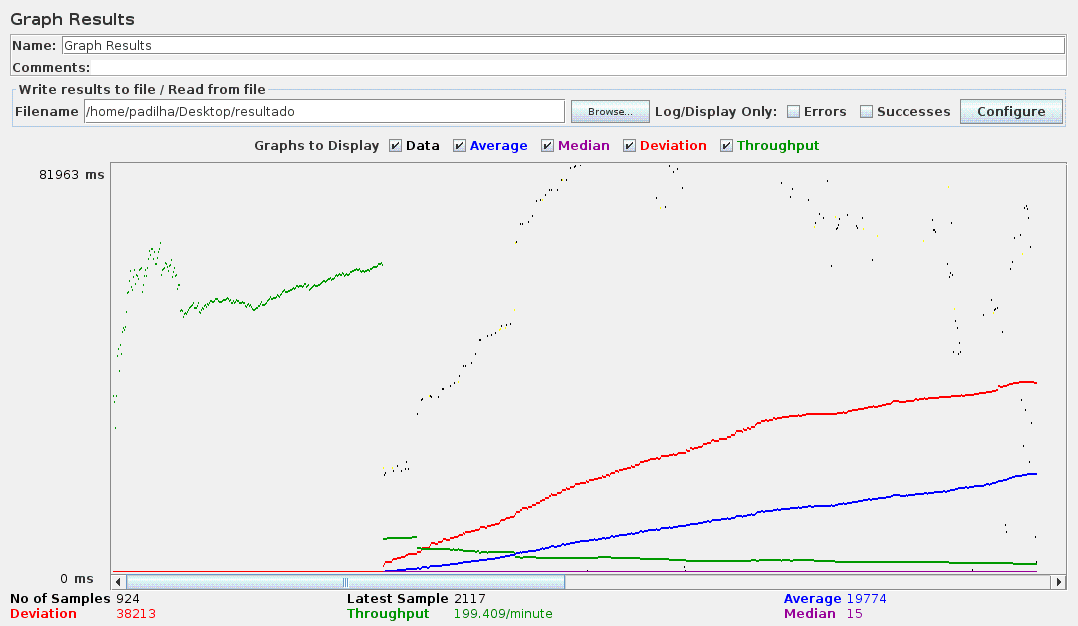
\includegraphics[width=\textwidth]{figuras/psy_90}}\\
\subfloat[MS SQL Server]{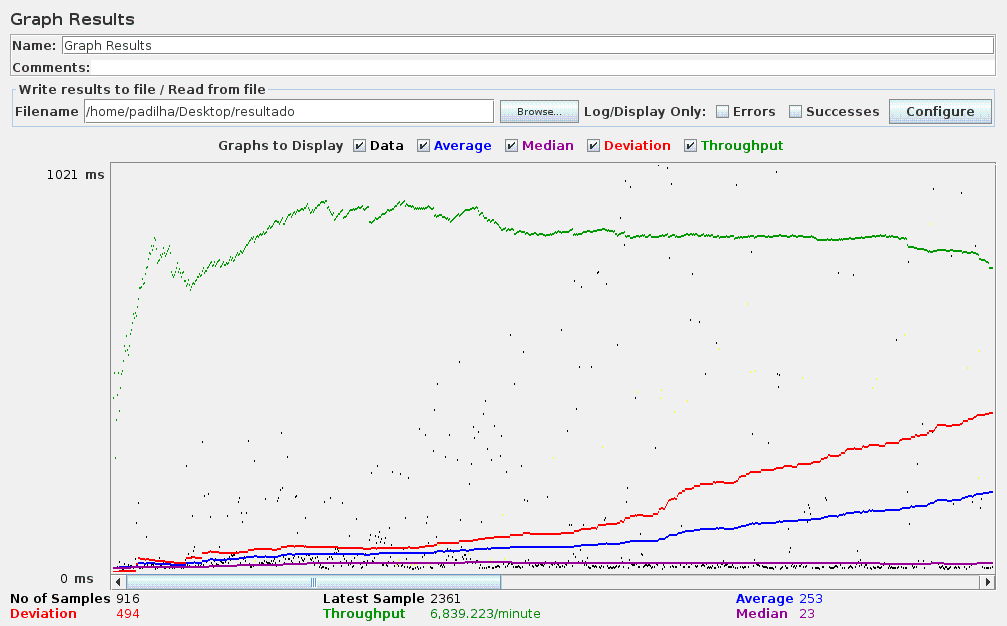
\includegraphics[width=\textwidth]{figuras/pms_90}}
\caption{Gráfico gerado pelo JMeter: 90 usuários}
\label{fig:comp_90}
\end{figure}

\begin{figure}[H]
\centering
\subfloat[Sybase ASE]{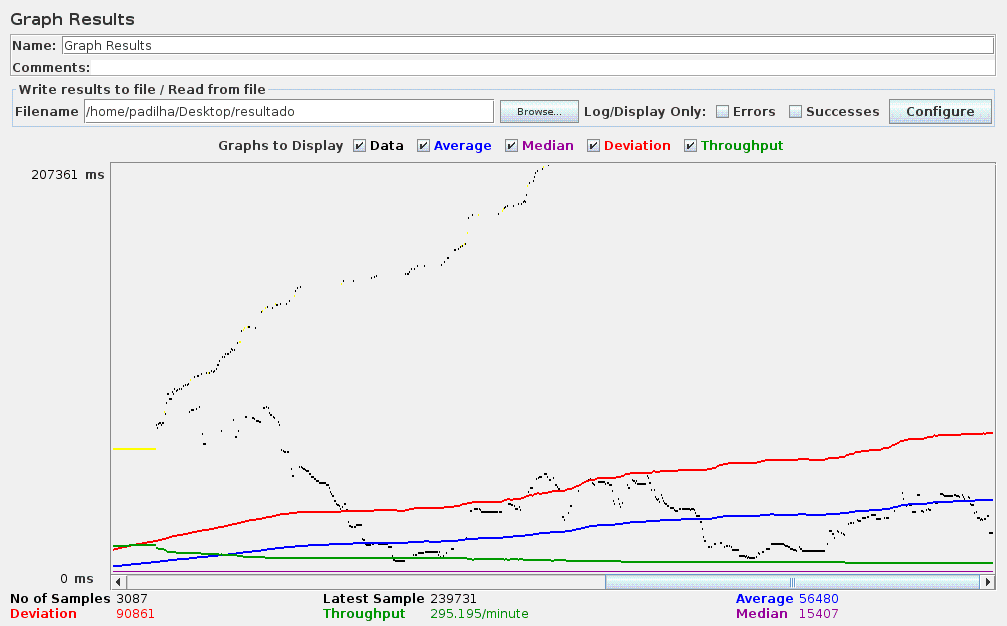
\includegraphics[width=\textwidth]{figuras/psy_360}}\\
\subfloat[MS SQL Server]{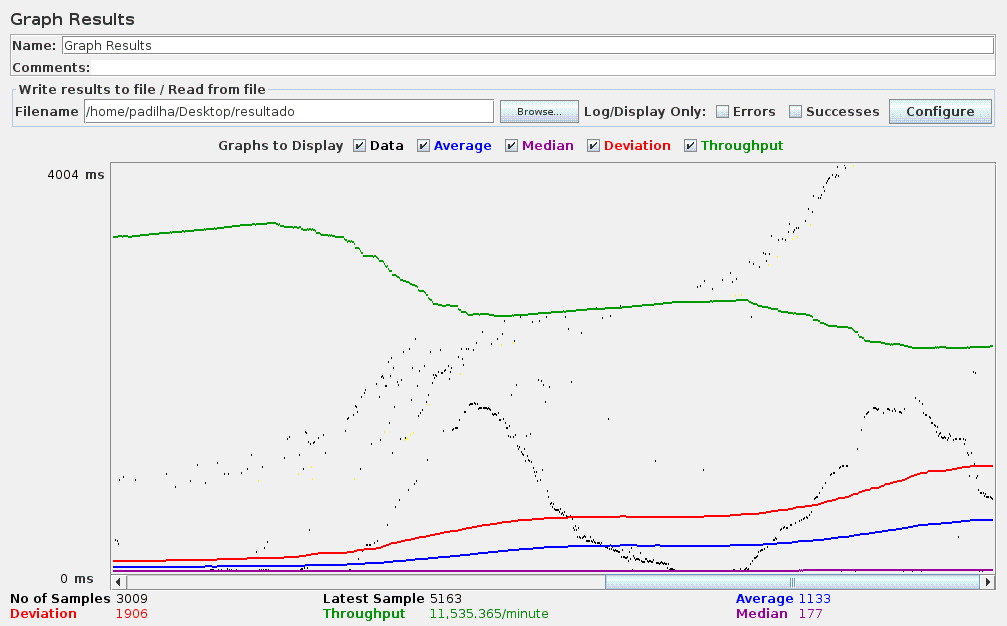
\includegraphics[width=\textwidth]{figuras/pms_360}}
\caption{Gráfico gerado pelo JMeter: 360 usuários}
\label{fig:comp_360}
\end{figure}


A linha verde nos gráficos indica a vazão de dados do servidor em transações por minuto, enquanto que as linhas vermelha, azul e lilás correspondem respectivamente ao desvio padrão, média e mediana do tempo de resposta das requisições.
\par

Analisando o tempo médio aproximado de resposta das requisições, tem-se que:

\begin{itemize}
\item 30 usuários~\ref{fig:comp_30}: 7,7s em Sybase e 80ms em MS SQL Server;
\item 90 usuários~\ref{fig:comp_90}: 19,7s em Sybase e 253ms em MS SQL Server;
\item 30 usuários~\ref{fig:comp_360}: 56,5s em Sybase e 1100ms em MS SQL Server;
\end{itemize}

\subsection{Conclusão dos testes}

Ao utilizar o banco de dados Sybase ASE no DataUSP-PósGrad não foi possível avaliar a escalabilidade dos Serviços Web REStful, uma vez que o Servidor de Recursos passou a maior parte do tempo ocioso, esperando dados do banco. Porém, ao utilizar-se o banco de dados Microsoft SQL Server que, apesar de na USP ser um banco de testes executado em uma máquina virtual, foi centenas de vezes mais rápido do que o Sybase ASE, fazendo com que o Servidor de Recursos esgotasse o processamento e também a memória ram da máquina onde foi executado nos testes.
\par
Não apenas o tempo de resposta das requisições foi consideravelmente menor no Microsoft SQL Server, como sua vazão de dados foi milhares de vezes maior, aumentando conforme o número de usuários simultâneos. O Sybase ASE, do contrário, manteve sua vazão ao longo de todos os testes, saturando sua capacidade com apenas 30 usuários simultâneos. 
\par
Apenas a título de curiosidade, foi feito um teste com dois mil usuários simultâneos (um pouco mais do que todos os usuários com acesso ao sistema). Com o Microsoft SQL Server o tempo médio de resposta do Servidor de Recursos foi de 5,2s. Ao utilizar o Sybase ASE não foi possível completar o teste pois, após alguns minutos de espera, o banco de dados repentinamente encerrava a conexão.
\par 
O uso do banco de dados Sybase ASE no DataUSP-PósGrad acarreta sérios problemas de desempenho em um cenário de alta demanda por seus serviços. Mesmo assim é o banco padrão de praticamente todos os outros sistemas administrativos da USP.

\chapter{Conclusões}
\label{ch:5}

Para se compreender a situação atual de uma instituição do tamanho da USP, é fundamental fazer uma análise
abrangente e precisa dos dados acumulados ao longo dos anos. É nesse contexto que surgiu o DataUSP-PósGrad como sistema analítico da pós-graduação da Universidade de São Paulo.

\par Os dois principais objetivos desse trabalho foram a criação de um Data Warehouse e um sistema baseado em Serviços Web para gerar relatórios sob demanda referentes aos dados da pós-graduação da USP. 

\par O Data Warehouse foi construído com dados de fontes internas, no caso dos dados dos programas, áreas e pessoas, e também de fontes externas, para se obter dados da produção acadêmica dos docentes e seu impacto na comunidade científica. As fontes internas são os dados coletados pelos demais sistemas administrativos da USP, por exemplo o sistema Janus, enquanto que as principais fontes externas são as páginas web do Google Scholar e também do Scopus.

\par Seguindo os conceitos da arquitetura REST, o sistema foi dividido em duas componentes: o Servidor de Recursos e a Interface Web. O Servidor de Recursos, que é propriamente o Serviço Web, foi implementado em Java por meio da biblioteca Jersey. Já a Interface Web, responsável por consumir os dados do Servidor de Recursos e construir os relatórios, foi implementada em JavaScript, por meio das bibliotecas JQuery e Fusion Charts, e HTML5. Além disso um sistema auxiliar escrito em Python, o Web Crawler, foi construído para obter informações da produção intelectual dos docentes da USP nas fontes de dados externas, além de integrá-las ao Data Warehouse.

\par Embora o DataUSP-PósGrad utilize o banco de dados Sybase ASE, como praticamente todos os sistemas da USP, utilizar uma arquitetura orientada a serviços provou-se bastante adequada para o ambiente USP. Desde que não haja um gargalo no banco de dados, esse modelo arquitetural garante alta escalabilidade de recursos computacionais e na implementação de novas funcionalidades. Facilita a comunicação e a integração com outros futuros Serviços Web e, ainda, definine um novo paradigma para se construir sistemas administrativos dentro da Universidade.

\par Os dados fornecidos pelo DataUSP-PósGrad são essenciais para se conhecer a evolução dos programas da pós-graduação, assim como para detectar tendências e manter o padrão de excelência dos cursos. Conseguir esses dados em tempo real é indispensável para agilizar a tomada de decisões e corrigir eventuais problemas, ou ainda entender alguma anomalia.

\par Com o sucesso do DataUSP-PósGrad a tendência é que apareçam novos sistemas na USP orientados a serviços, e até mesmo a modernização de sistemas já existentes, aumentando o foco nos dados e de como eles representam o estado dos processos administrativos.


\addcontentsline{toc}{chapter}{\numberline{}Bibliografia}
\begin{thebibliography}{99}

\bibitem{J0} John Ousterhout, The RAMCloud Project, 2015\\
\mbox{}\hfill\texttt{\url{https://ramcloud.atlassian.net/wiki/display/RAM/RAMCloud}}

\bibitem{J1} John Ousterhout, The RAMCloud Storage System, 2014\\
\mbox{}\hfill\texttt{\url{https://ramcloud.atlassian.net/wiki/download/attachments/6848571/RAMCloudPaper.pdf}}

\bibitem{J2} John Ousterhout, The Case for RAMCloud, 2011\\
\mbox{}\hfill\texttt{\url{http://portal.acm.org/citation.cfm?id=1965751}}

\bibitem{J3} John Ousterhout, A collection of all of John Ousterhout's RAMCloud slides, 2012\\
\mbox{}\hfill\texttt{\url{https://ramcloud.atlassian.net/wiki/display/RAM/RAMCloud+Presentations}}

\bibitem{J4} John Ousterhout, Introductory talk on RAMCloud, 2011\\
\mbox{}\hfill\texttt{\url{http://www.youtube.com/watch?v=lcUvU3b5co8}}


\end{thebibliography}


\end{document}
